
%%%%%%%%%%%%%%%%%%%% author.tex %%%%%%%%%%%%%%%%%%%%%%%%%%%%%%%%%%%
%
% sample root file for your "contribution" to a contributed volume
%
% Use this file as a template for your own input.
%
%%%%%%%%%%%%%%%% Springer %%%%%%%%%%%%%%%%%%%%%%%%%%%%%%%%%%


% RECOMMENDED %%%%%%%%%%%%%%%%%%%%%%%%%%%%%%%%%%%%%%%%%%%%%%%%%%%

\documentclass[graybox]{svmult}

% choose options for [] as required from the list
% in the Reference Guide

\usepackage{mathptmx}       % selects Times Roman as basic font
\usepackage{helvet}         % selects Helvetica as sans-serif font
\usepackage{courier}        % selects Courier as typewriter font
\usepackage{type1cm}        % activate if the above 3 fonts are
                            % not available on your system
%
\usepackage{makeidx}         % allows index generation
\usepackage{wrapfig}
\usepackage{graphicx}        % standard LaTeX graphics tool
                             % when including figure files
\usepackage{multicol}        % used for the two-column index
\usepackage[bottom]{footmisc}% places footnotes at page bottom
\usepackage{marginnote}
\newcommand{\TODO}[1]{\marginnote{TODO: #1}}    % TODO Befehl
\usepackage{units,amsmath}
\usepackage{todonotes}
\usepackage{hyperref}
\hypersetup{
    colorlinks=true,
    linkcolor=blue,
    filecolor=magenta,      
    urlcolor=cyan,
}
\usepackage{url}
\usepackage{siunitx}
\usepackage{units}
\usepackage{subcaption}
% see the list of further useful packages
% in the Reference Guide

\makeindex             % used for the subject index
                       % please use the style svind.ist with
                       % your makeindex program

%\usepackage{cleveref}[2012/02/15]
%\crefformat{footnote}{#2\footnotemark[#1]#3}

\renewcommand{\O}{{\cal O}}
\renewcommand{\leadsto}{\rightsquigarrow}
\newcommand{\V}[1]{\text{\boldmath $#1$}}    % Format for "Vector"
\newcommand{\M}[1]{\V{#1}}                   % Format for "Matrix"

\newcommand{\R}{\mathbbm{R}}                 % set of real number
\newcommand{\N}{\mathbbm{N}}                 % set of natural numbers
\newcommand{\C}{\mathbbm{C}}                 % ...
\newcommand{\1}{\mathbbm{1}}                 % identity matrix


%%%%%%%%%%%%%%%%%%%%%%%%%%%%%%%%%%%%%%%%%%%%%%%%%%%%%%%%%%%%%%%%%%%%%%%%%%%%%%%%%%%%%%%%%

%%
% Motivation, Problem Statement, Related Work (one page)
% Technical Approach (one page)
% Results (one page)
% Experiments completed or scheduled (one page)
% Main experimental insights (one page)
% References (one page)
%%

\begin{document}

\title*{Extended Abstract:           L.U.N.A. - A Laser-Mapping Unidirectional Navigation Actuator} 
\author{Jasper Zevering, Anton Bredenbeck, Fabian Arzberger,
  Dorit Borrmann and Andreas N\"uchter}
% FIXME sort the authors
% Use \authorrunning{Short Title} for an abbreviated version of
% your contribution title if the original one is too long

%\and Name of Second Author \at Name, Address of Institute 
%\email{name@email.address}

%
% Use the package "url.sty" to avoid
% problems with special characters
% used in your e-mail or web address
%
\maketitle

%\abstract*{Each chapter should be preceded by an abstract (10--15 lines long) 
%that summarizes the content. The abstract will appear \textit{online} at 
%\url{www.SpringerLink.com} and be available with unrestricted access. This 
%allows unregistered users to read the abstract as a teaser for the complete 
%chapter. As a general rule the abstracts will not appear in the printed 
%version 
%of your book unless it is the style of your particular book or that of the 
%series to which your book belongs.
%Please use the 'starred' version of the new Springer \texttt{abstract} command 
%for typesetting the text of the online abstracts (cf. source file of this 
%chapter template \texttt{abstract}) and include them with the source files of 
%your manuscript. Use the plain \texttt{abstract} command if the abstract is 
%also to appear in the printed version of the book.}

\section{Motivation, Problem Statement, Related Work}

To foster new advances in the latter, specifically for underground environments, the  Defense Advanced Research Projects Agency (DARPA) of the US Defense Department established the yearly ``SubT'' Challenge in 2017.
In this challenge, teams are tasked to ``Drive novel approaches and technologies to allow warfighters and first-responders to rapidly map, navigate, and search dynamic underground environments.''~\cite{allen} proving the demand for further research in this domain.
One subtask of this challenge is building an accurate 3D model of the environment, i.e., mapping the surroundings. 
This paper shows a proof of concept of a such a novel approach and validates it with experiments.

One such approach using a 2D laser scanner to scan 3D indoor environments has been proposed in~\cite{classical_mechanics_scanner}.
The authors mount a 2D laser scanner on a cylindrical structure.
An operator then initiates a rolling motion by manually pushing the contraption.
This enables the scanner to sense the 3D environment successfully.
However, manually pushing the scanner is not practical, especially for long scans.

Previous work includes our RADLER (RADial LasER scanning device), which consists of a 2D laser scanner attached to the axle of a unicycle~\cite{ISER2018}.
An operator pushes the unicycle along a requested path.
The inherent rotation of the wheel creates a radial 3D laser scanning pattern.
However, this approach still requires an operator, therefore does not fulfill the autonomy requirements. 

A more autonomous approach was taken by Fang et al.~\cite{3D_per_2D_based}.
The authors mounted a rotating 2D laser-scanner on top of a turtle-bot thus removing the need of an operator.
In contrast to the RADLER however, the turtle-bot does not provide an inherent rotation.
Therefore an additional actuator is required to create the radial 3D scanning-pattern. 

This paper builds upon the results of the RADLER and has a specific application of mapping lunar craters autonomously in mind.
We propose a novel approach to low-cost 3D laser scanning using a 2D laser scanner inside a spherical robot based on impulse by conversation of angular momentum (IBCOAM): the L.U.N.A. - sphere (Laser-mapping Unidirectional Navigation Actuator).
The 2D laser scanner is fixed to the spherical structure, hence a similar situation as with the RADLER is given: the inherent rotation of the sphere creates a radial 3D scanning pattern.
Using the format of a spherical robot permits the system to be designed more compact. 
Additionally, the spherical shell doubles as a protective layer for the actuators, sensors and electronics. 
This is especially valuable for applications in rough terrain or scenarios in which non-minimal impact is expected, such as space applications.
During a launch, withstanding large G-forces is a necessary requirement, which can be better implemented using the spherical format. 
Furthermore, an operator is no longer required given a drive implemented in the robot.

\section{Technical Approach}
\label{sec:TechnicalApproach}

\begin{figure}
\centering
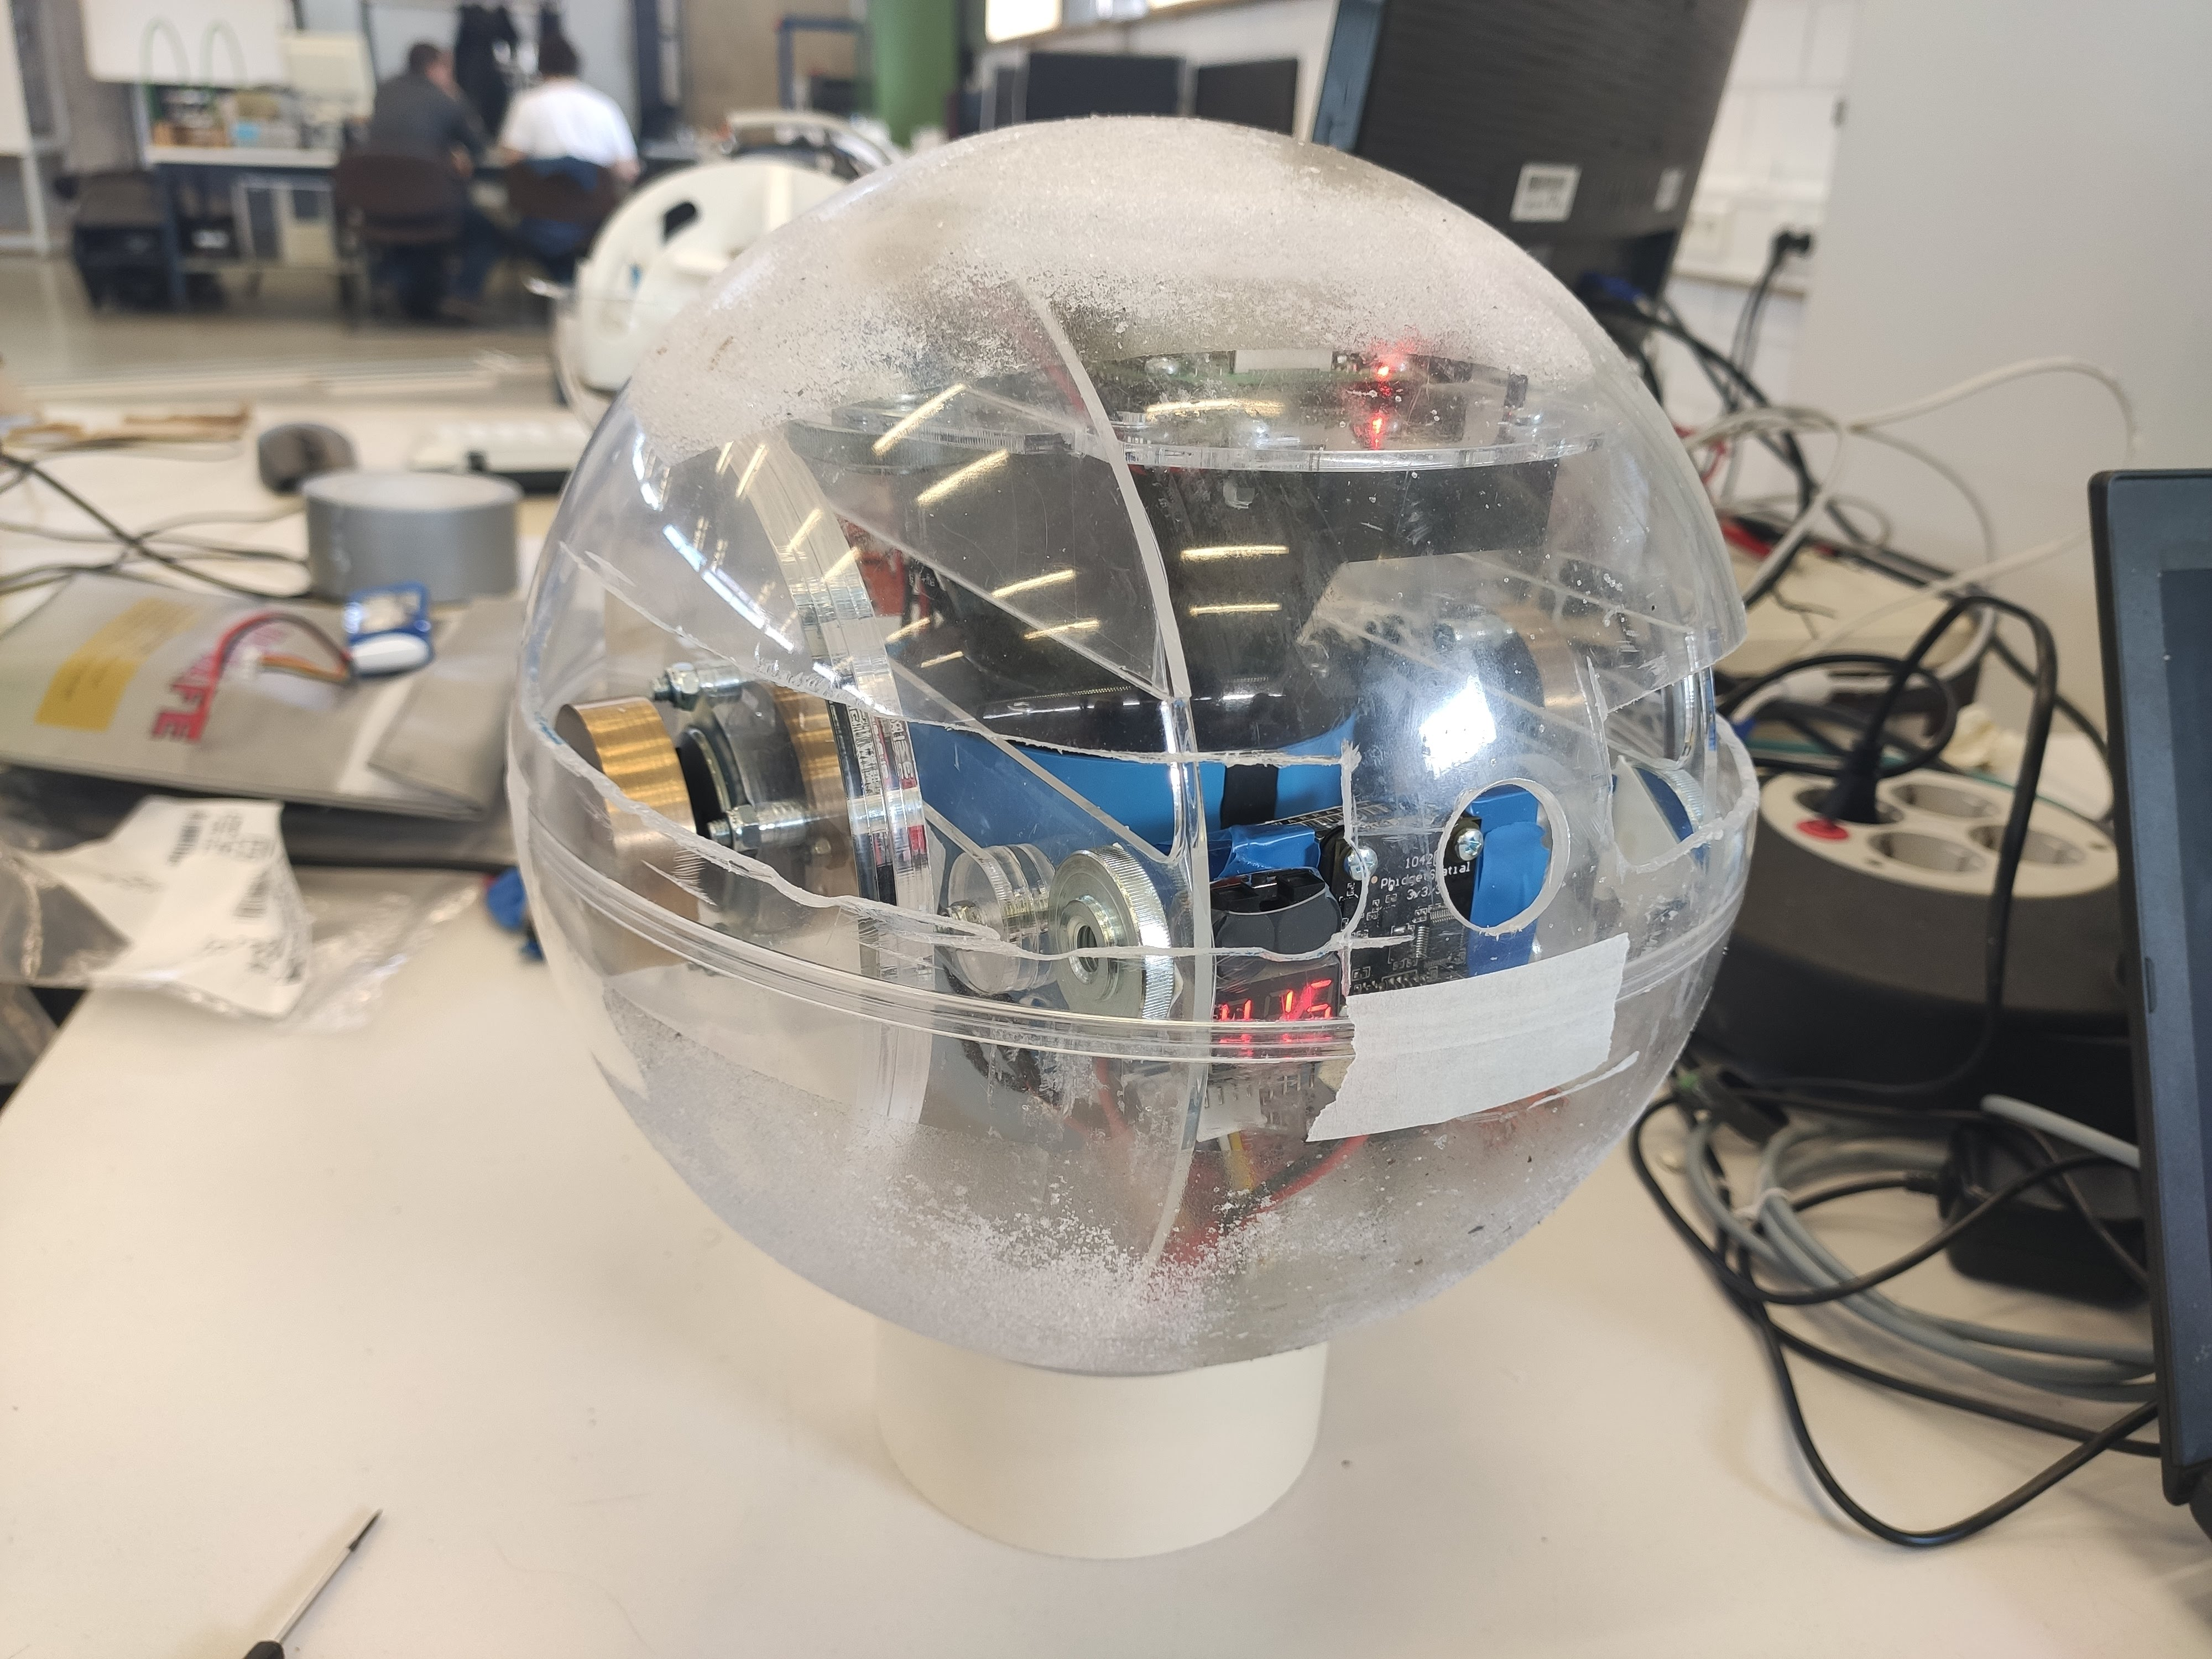
\includegraphics[height=50mm]{../Media/sphereFullshellLeft.jpg}
\hfill
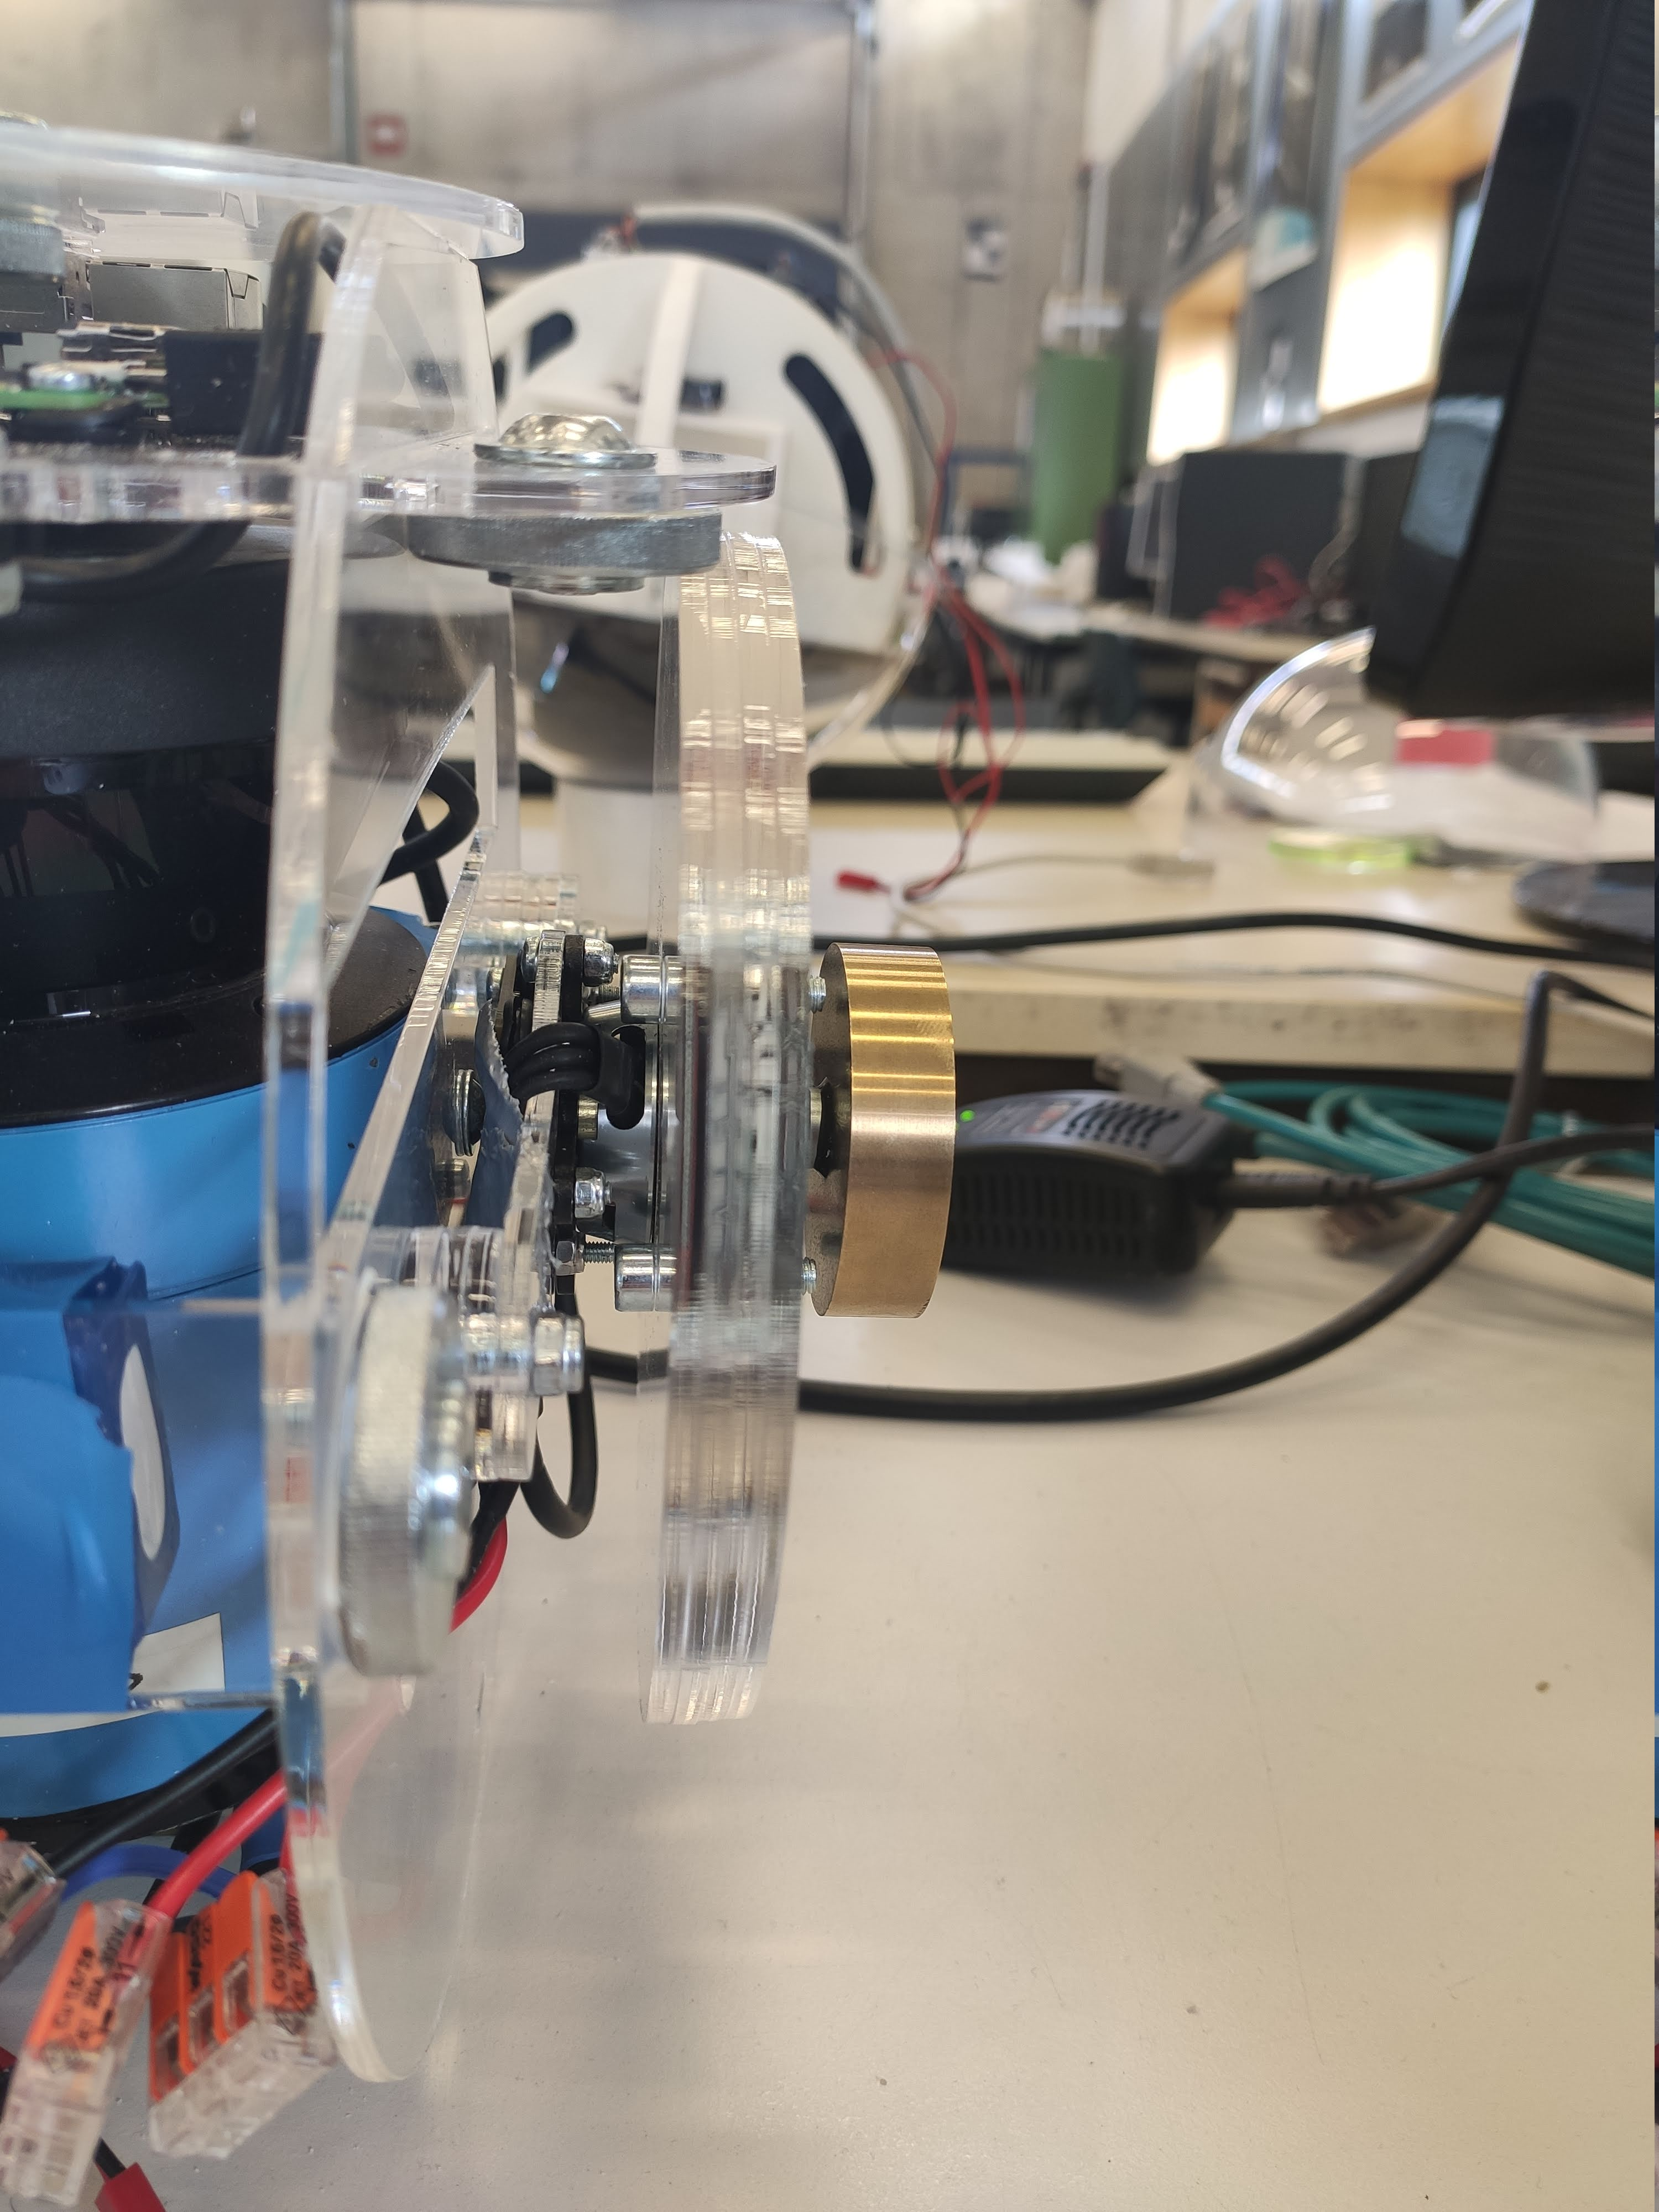
\includegraphics[height=50mm]{../Media/sphereRightMotor.jpg}   
\label{sec:TechnicalApproach:fig:motor}
\label{sec:TechnicalApproach:fig:prototype}
\caption{Hardware setup of the L.U.N.A sphere prototype, including notches in the shell and friction granule. IMU (beneath supporting structure) and brushless motor (above supporting structure) of the L.U.N.A sphere without shell, including flywheel mass. Hardware setup of the L.U.N.A sphere prototype, including notches in the shell and friction granule.}
\end{figure}

\todo{Bilder mit hoehe anpassen, keine captions in subfigures, optimale mm werte finden, caption anpassen (left / right) }

\todo{Wie dreht sich die Kugel überhaupt ? COAM + Cubli paper lesen / gyro effekt + video schneiden (ohne ton) }

Figure \ref{sec:TechnicalApproach:fig:prototype} shows the final hardware setup of the robot.
\todo{was ist da drinnen (raspberry pi, ..), wo ist es da drinnen, warum ist es da drinnen.}
In order to reduce complexity with respect to the 3D-transformation calculations, the laserscanner was placed at the center of a spherical acrylic glass shell as precisely as possible.
This limits the laser scanners movement to rotational movement and removes translational movement completely. With this initial setup given, the only room left for the acrylic glass structural components, batteries, boardcomputer, IMUs, motors, weights and wiring are the spaces between the scanner and the shell.
Figure \ref{sec:TechnicalApproach:fig:motor} shows one Turnigy Park480 brushless outrunner motor \cite{turnigymotor} of the COAM drive with two flywheels attached.
Strong epoxy glue attaches the weights to the motor shafts and shells.
As the flywheels start spinning with respect to the structural components of the sphere, the sphere itself starts spinning with respect to the ground. 

Figure \ref{sec:TechnicalApproach:fig:prototype} also shows that the top and the bottom of the shell are covered in table salt, which made a good granule to increase friction to the ground in the early testing phase. Furthermore, there are notches in the front side of the shell to increase permeability for the laser.
Unfortunately, the laser scanner measurements are still affected by blockades due to components of the sphere.
Specifically, the outside shell is an inhibiting factor as an object with the distance of the radius is measured at all times, \todo{which is why measurement slits}
                                                                                                                                                                                                                  
\begin{figure}                                                                                                                                                                                                    
\centering                                                                                                                                                                                                        
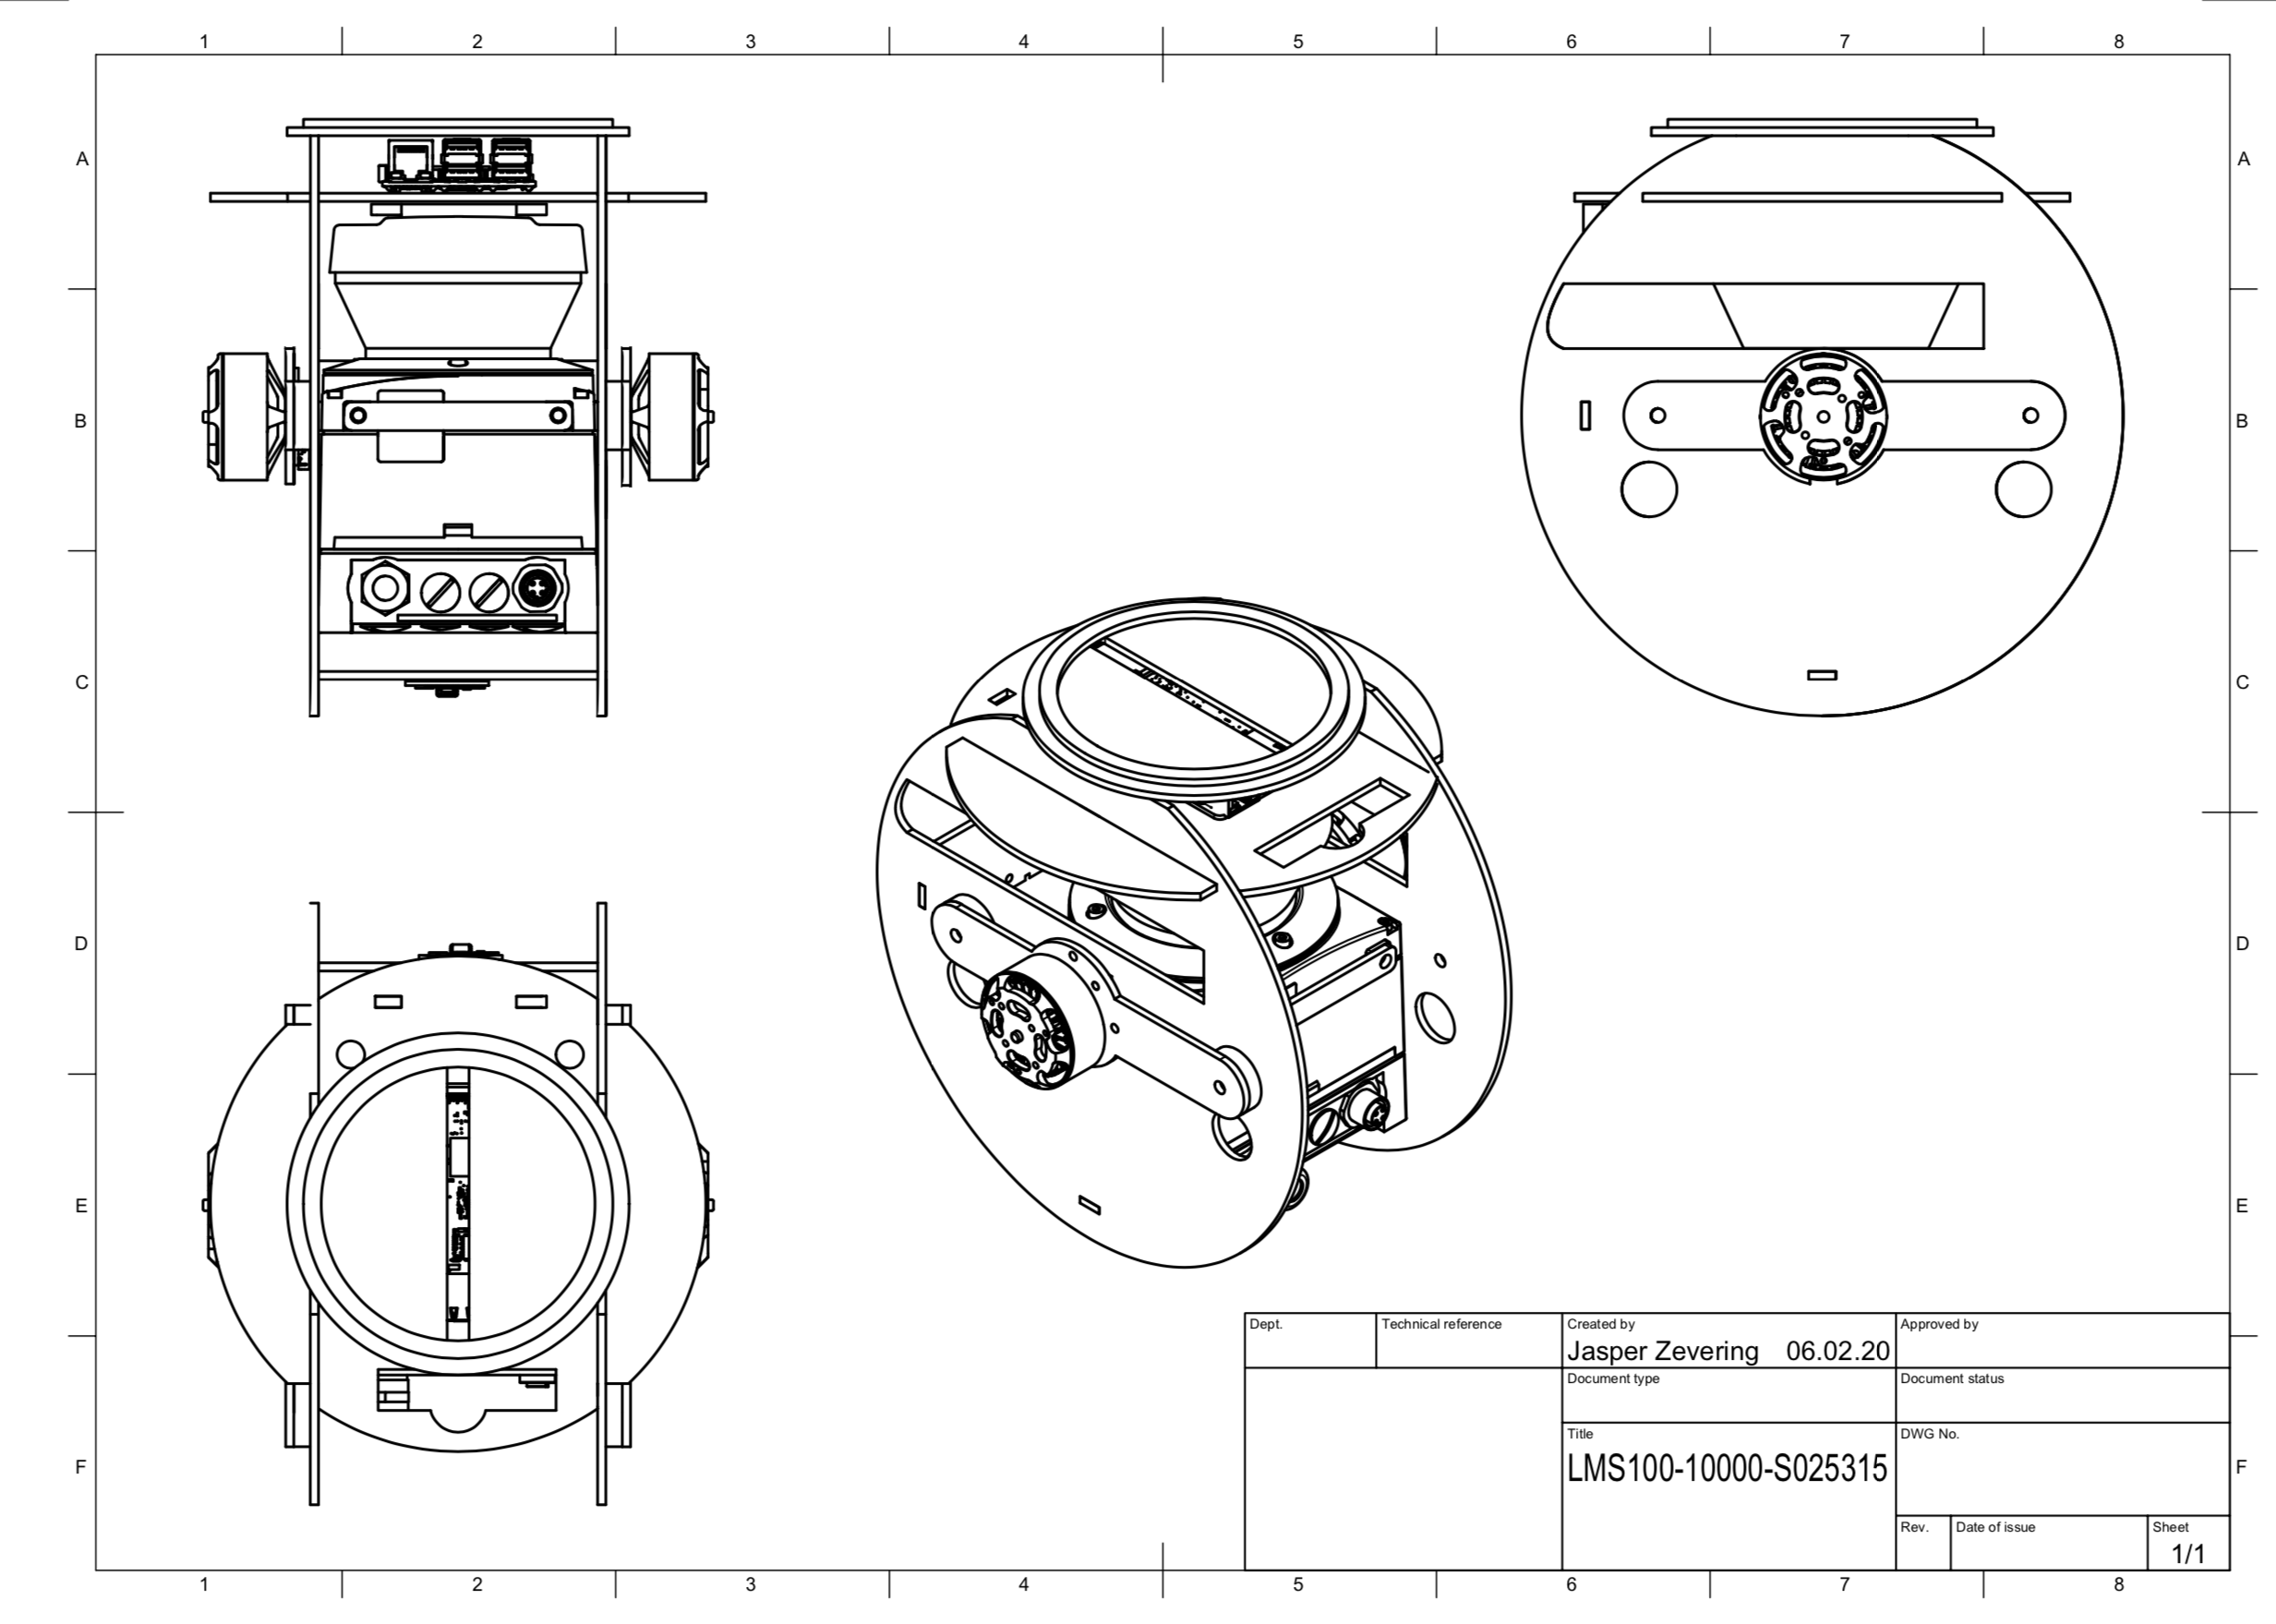
\includegraphics[width=\textwidth]{../Media/BlueprintPNG.png}                                                                                                                                                      
\caption{Blueprint of the mechanical structure of the spherical robot.}                                                                                                                                   
\label{sec:TechnicalApproach:fig:blueprint}                                                                                                                                                                       
\end{figure}                                                                                                                                                                                                      
                                                                                                                                                                                                                  
Figure \ref{sec:TechnicalApproach:fig:blueprint} shows a CAD blueprint of the overall interior layout of the mechanical structure of the L.U.N.A sphere, ignoring the outside sphere, flywheels and wiring.
The payload is mounted to supporting structural components which are made of acrylic glass.
The Raspberry Pi 3B boardcomputer is placed on top of the laser.
Above that, another supporting structure holds additional counterweights to correct for inhomogeneous weight distribution.                                                                                                     
The battery finds its place in front of the laser scanner on another supporting structure.
The two brushless motors were each placed on one side of the supporting structure with spacers that leave room for the side IMU underneath one of the motors.
Two other IMUs are placed in front of and beneath the laser to ensure coverage of all axes.                                                                                 

\begin{figure}                                                                                                                                                                                                    
\centering
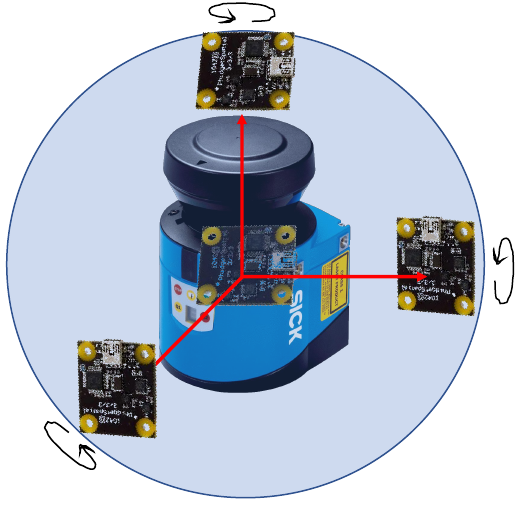
\includegraphics[width=0.5\textwidth]{../Media/virtualIMU.png}                                                                                                                                                      
\caption{Sketch that helps illustrate the combination of 3 IMUs into 1 virtual IMU that simulates being at the center of the sphere.}                                                                                                                           
\label{sec:SensorIntegration:fig:virtual}                                                                                                                                                                       
\end{figure}                                                                                                                                                                                                      

\subsection{Sensor Integration}
\label{sec:TechnicalApproach:sensorintegration}

The sensor integration is fully implemented with the Robot Operating System (ROS) using the Ubuntu distribution \href{http://wiki.ros.org/ROSberryPi}{ROSberryPi} which contains a pre-installed ROS version.
Overall, three seperate PhidgetsSpacial 10441B IMUs \cite{imuphidgets} keep track of the pose of the sphere.
Figure \ref{sec:SensorIntegration:fig:virtual} illustrates why three IMUs are used instead of just one.
\todo{Mehr erklären}
Previous prototypes have shown that transforming the data of only one non-centered IMU leads to lower quality measurements. \todo{die neue figure mit daten}
However, combining the measurements of three IMUs, where each of which measures only the static rotation around one of their rotational axes (which also represents a rotation axis of the sphere), leads to less noise.
Each IMU is perpendicular to the other two, so combining the axis measurements leads to a "virtual" IMU, which simulates being an IMU positioned at the center of the sphere. 

The IMUs also ship with accelerometers that are used to determine the full pose of the sphere.
Each IMU calculates their pose separately, using a quaternion extended Kalman filter (QEKF).
However, combining those poses into one does not have any positive effect, but only makes the software more resource demanding and slow.
Thus only the pose of the bottom IMU's accelerometer is used to keep track of the pose.

The motors are controlled using the piGPIO library. The GPIO signals are forwarded by the pins to two ESCs that drive the motors. 

Unfortunately, the brass weights are not drilled in the very center, causing an unbalance when rotating.
The resulting vibrations inhibit the movement of the sphere.
Thus a controller was implemented that measures the extend of the vibrations using standard deviations of the non-rotating axes of the IMU and adjusts the throttle of the motors accordingly.
This was done with a two-point controller with hysteresis.
Considering the translational velocity of the sphere in a controller is not possible.
The speed of the sphere is calculated by the rotational speed, which is why slippage of the sphere causes such a controller not to produce the desired motion. 

\subsection{Point Cloud Processing}                                                                                                                                                                                  
\label{sec:TechnicalApproach:pointcloudprocessing}
For the processing of the point cloud the 3D Toolkit (3DTK) was used.
This provides multiple methods and algorithms for processing 3D point clouds, especially the 6D continuous time Simultaneous Localization And Mapping (SLAM) algorithm (see \cite{3DARCH2017_1, LS2019}) as post-processing.
Therefore only the time-stamped raw data of the IMUs and laser-scanner is transferred and the estimation of the pose and the SLAM algorithm itself is performed externally.
For this prototype the transfer is realized using the host-function of ROS, giving the external PC the possibility to subscribe to the topics and process them.
3DTK itself takes pairs of files, one representing the pose, one the laser scanner data, and each file named by the time-stamp with an identifier if it is scan-data or pose.
Also, the use of USB-connected IMUs and ROS as transfer-mechanism of data leaves potential for enhancement and therefore reducing the load of the internal controller.
\section*{Results}
\label{sec:Results}

As proof of concept, the prototype of L.U.N.A sphere for 3D mapping using the concept impulse out of conservation of angular momentum as a unidirectional drive to roll a 2D laser scanner in an IMU equipped, pose-tracked spherical robot system, has been build and tested successfully. Potential for improvement and technical limitations have been identified.
The resulting sphere is shown in fig. \ref{sec:TechnicalApproach:fig:setup}
\begin{figure}
\centering                                                                                                                                                                                                        
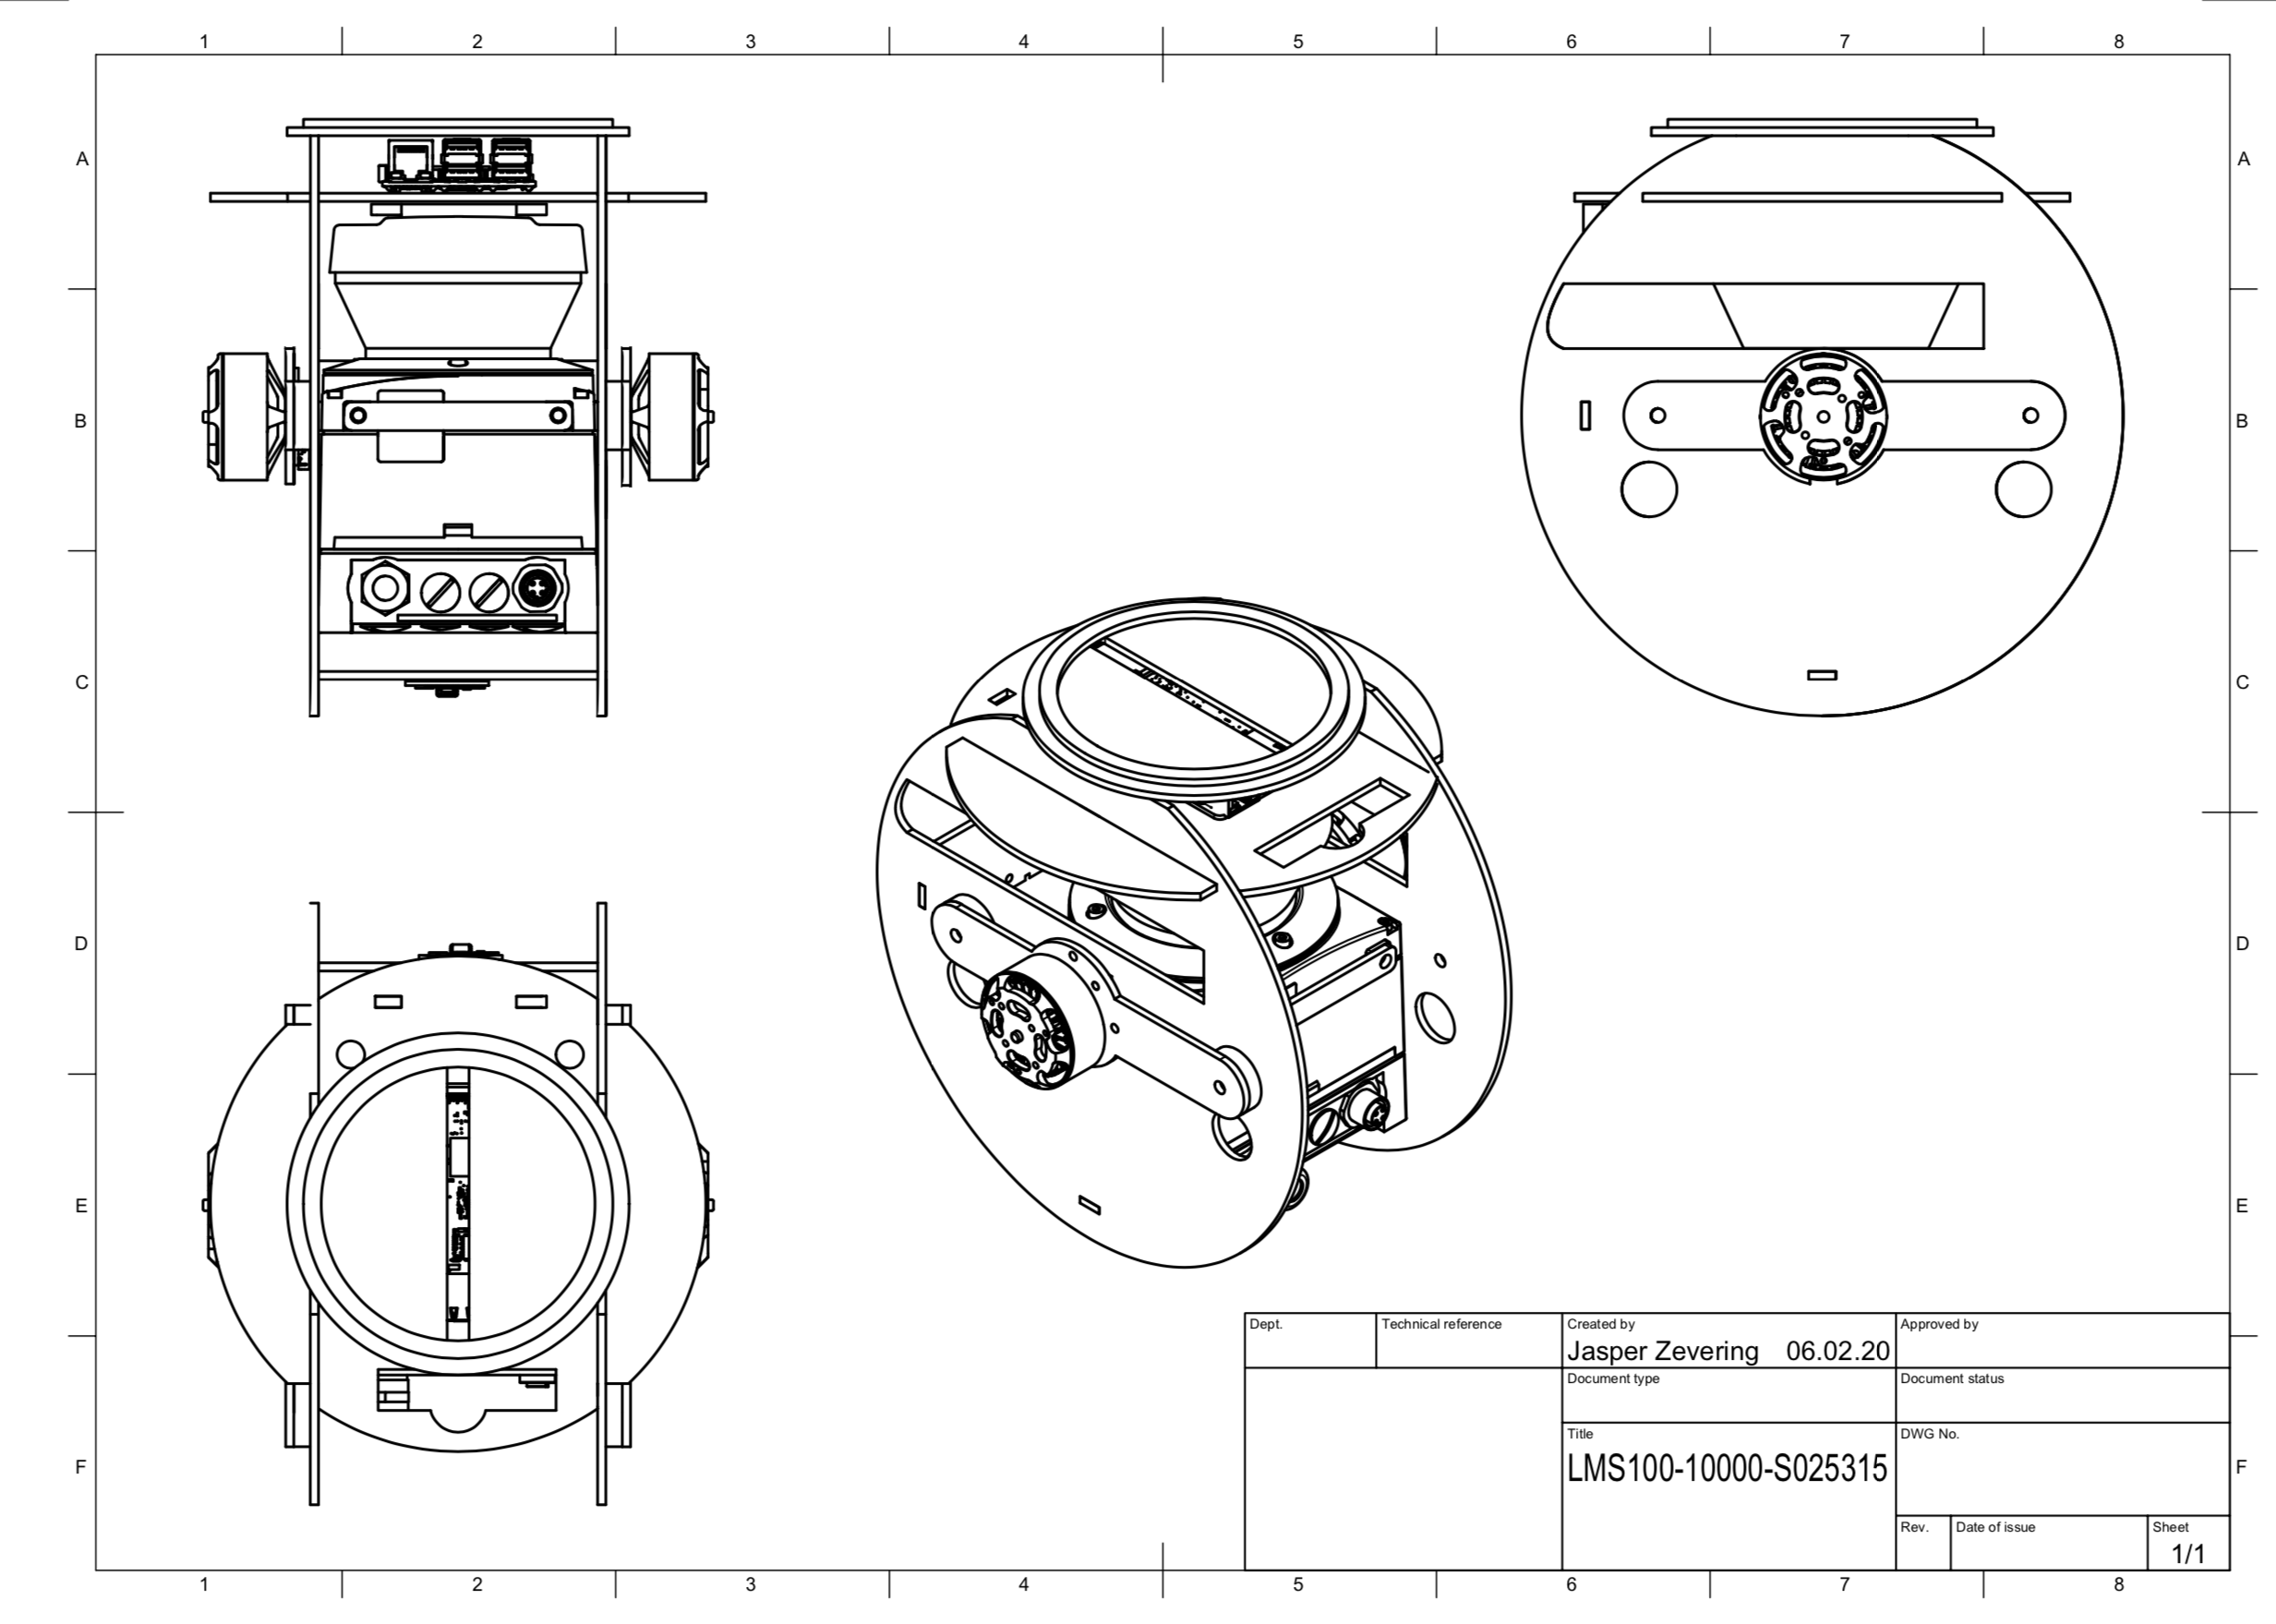
\includegraphics[height=50mm]{../Media/BlueprintPNG.png}                                                                                                                                                      \\
\vspace{0.5cm}
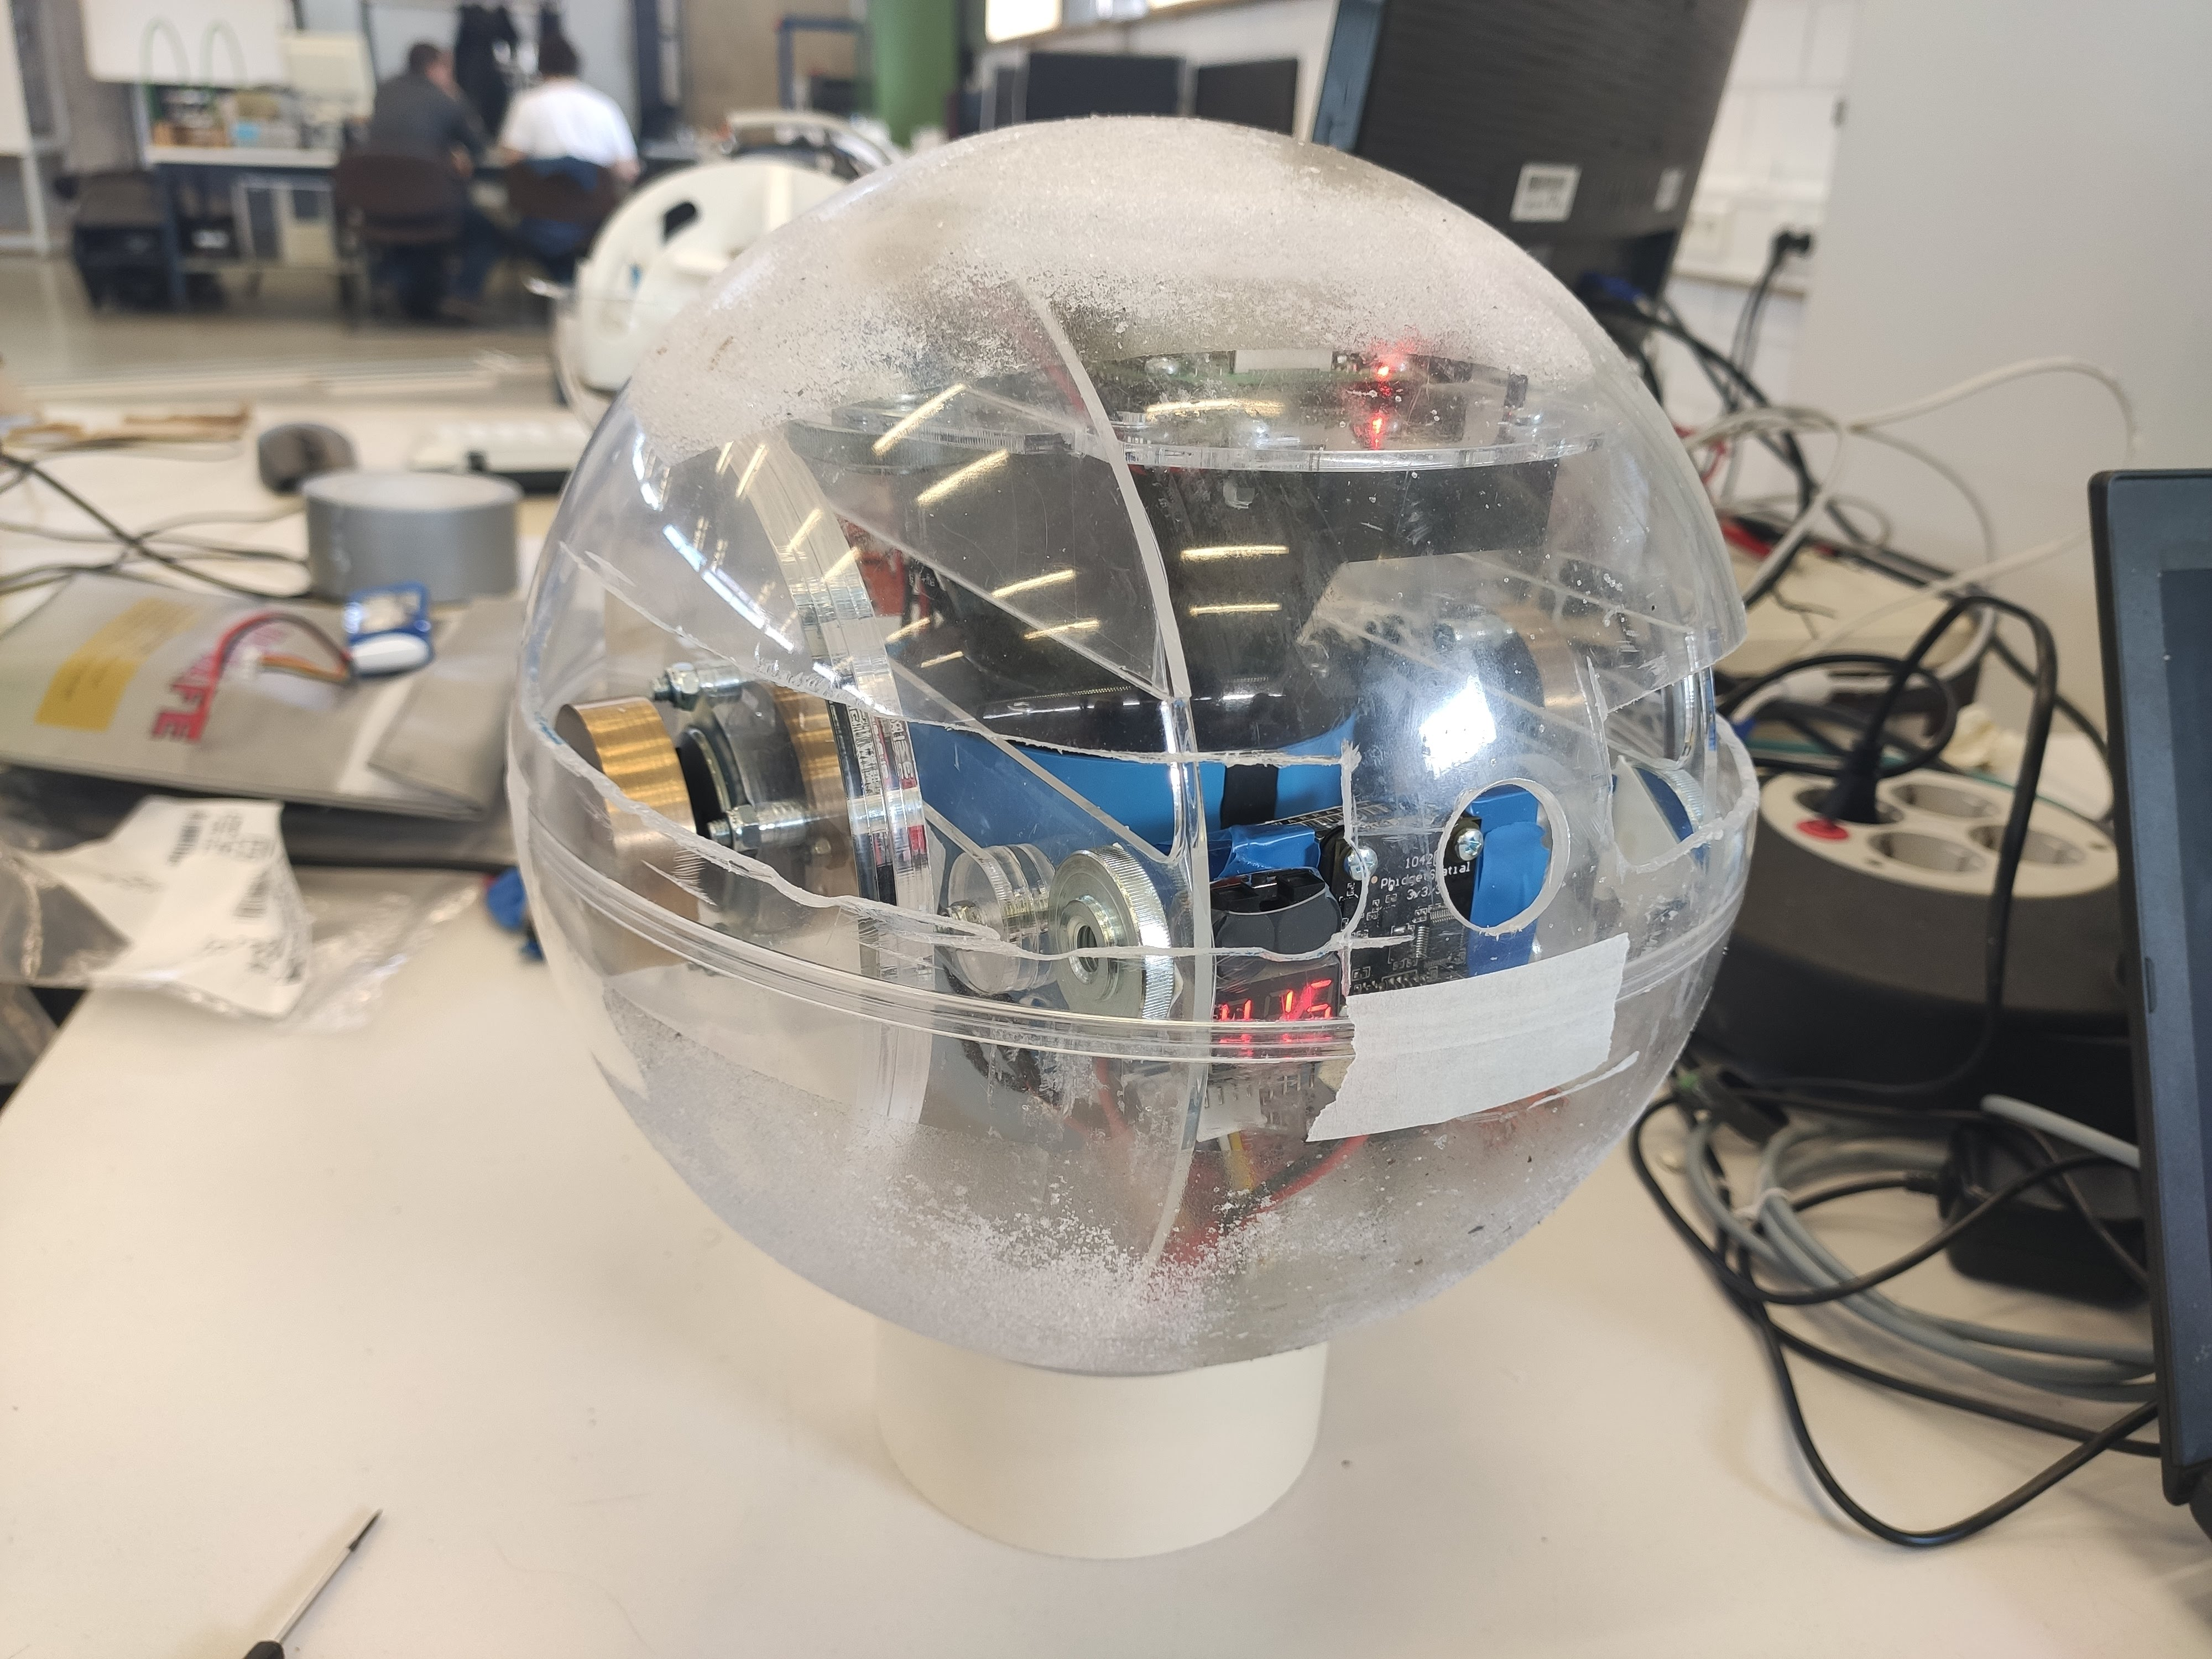
\includegraphics[height=50mm]{../Media/sphereFullshellLeft.jpg}
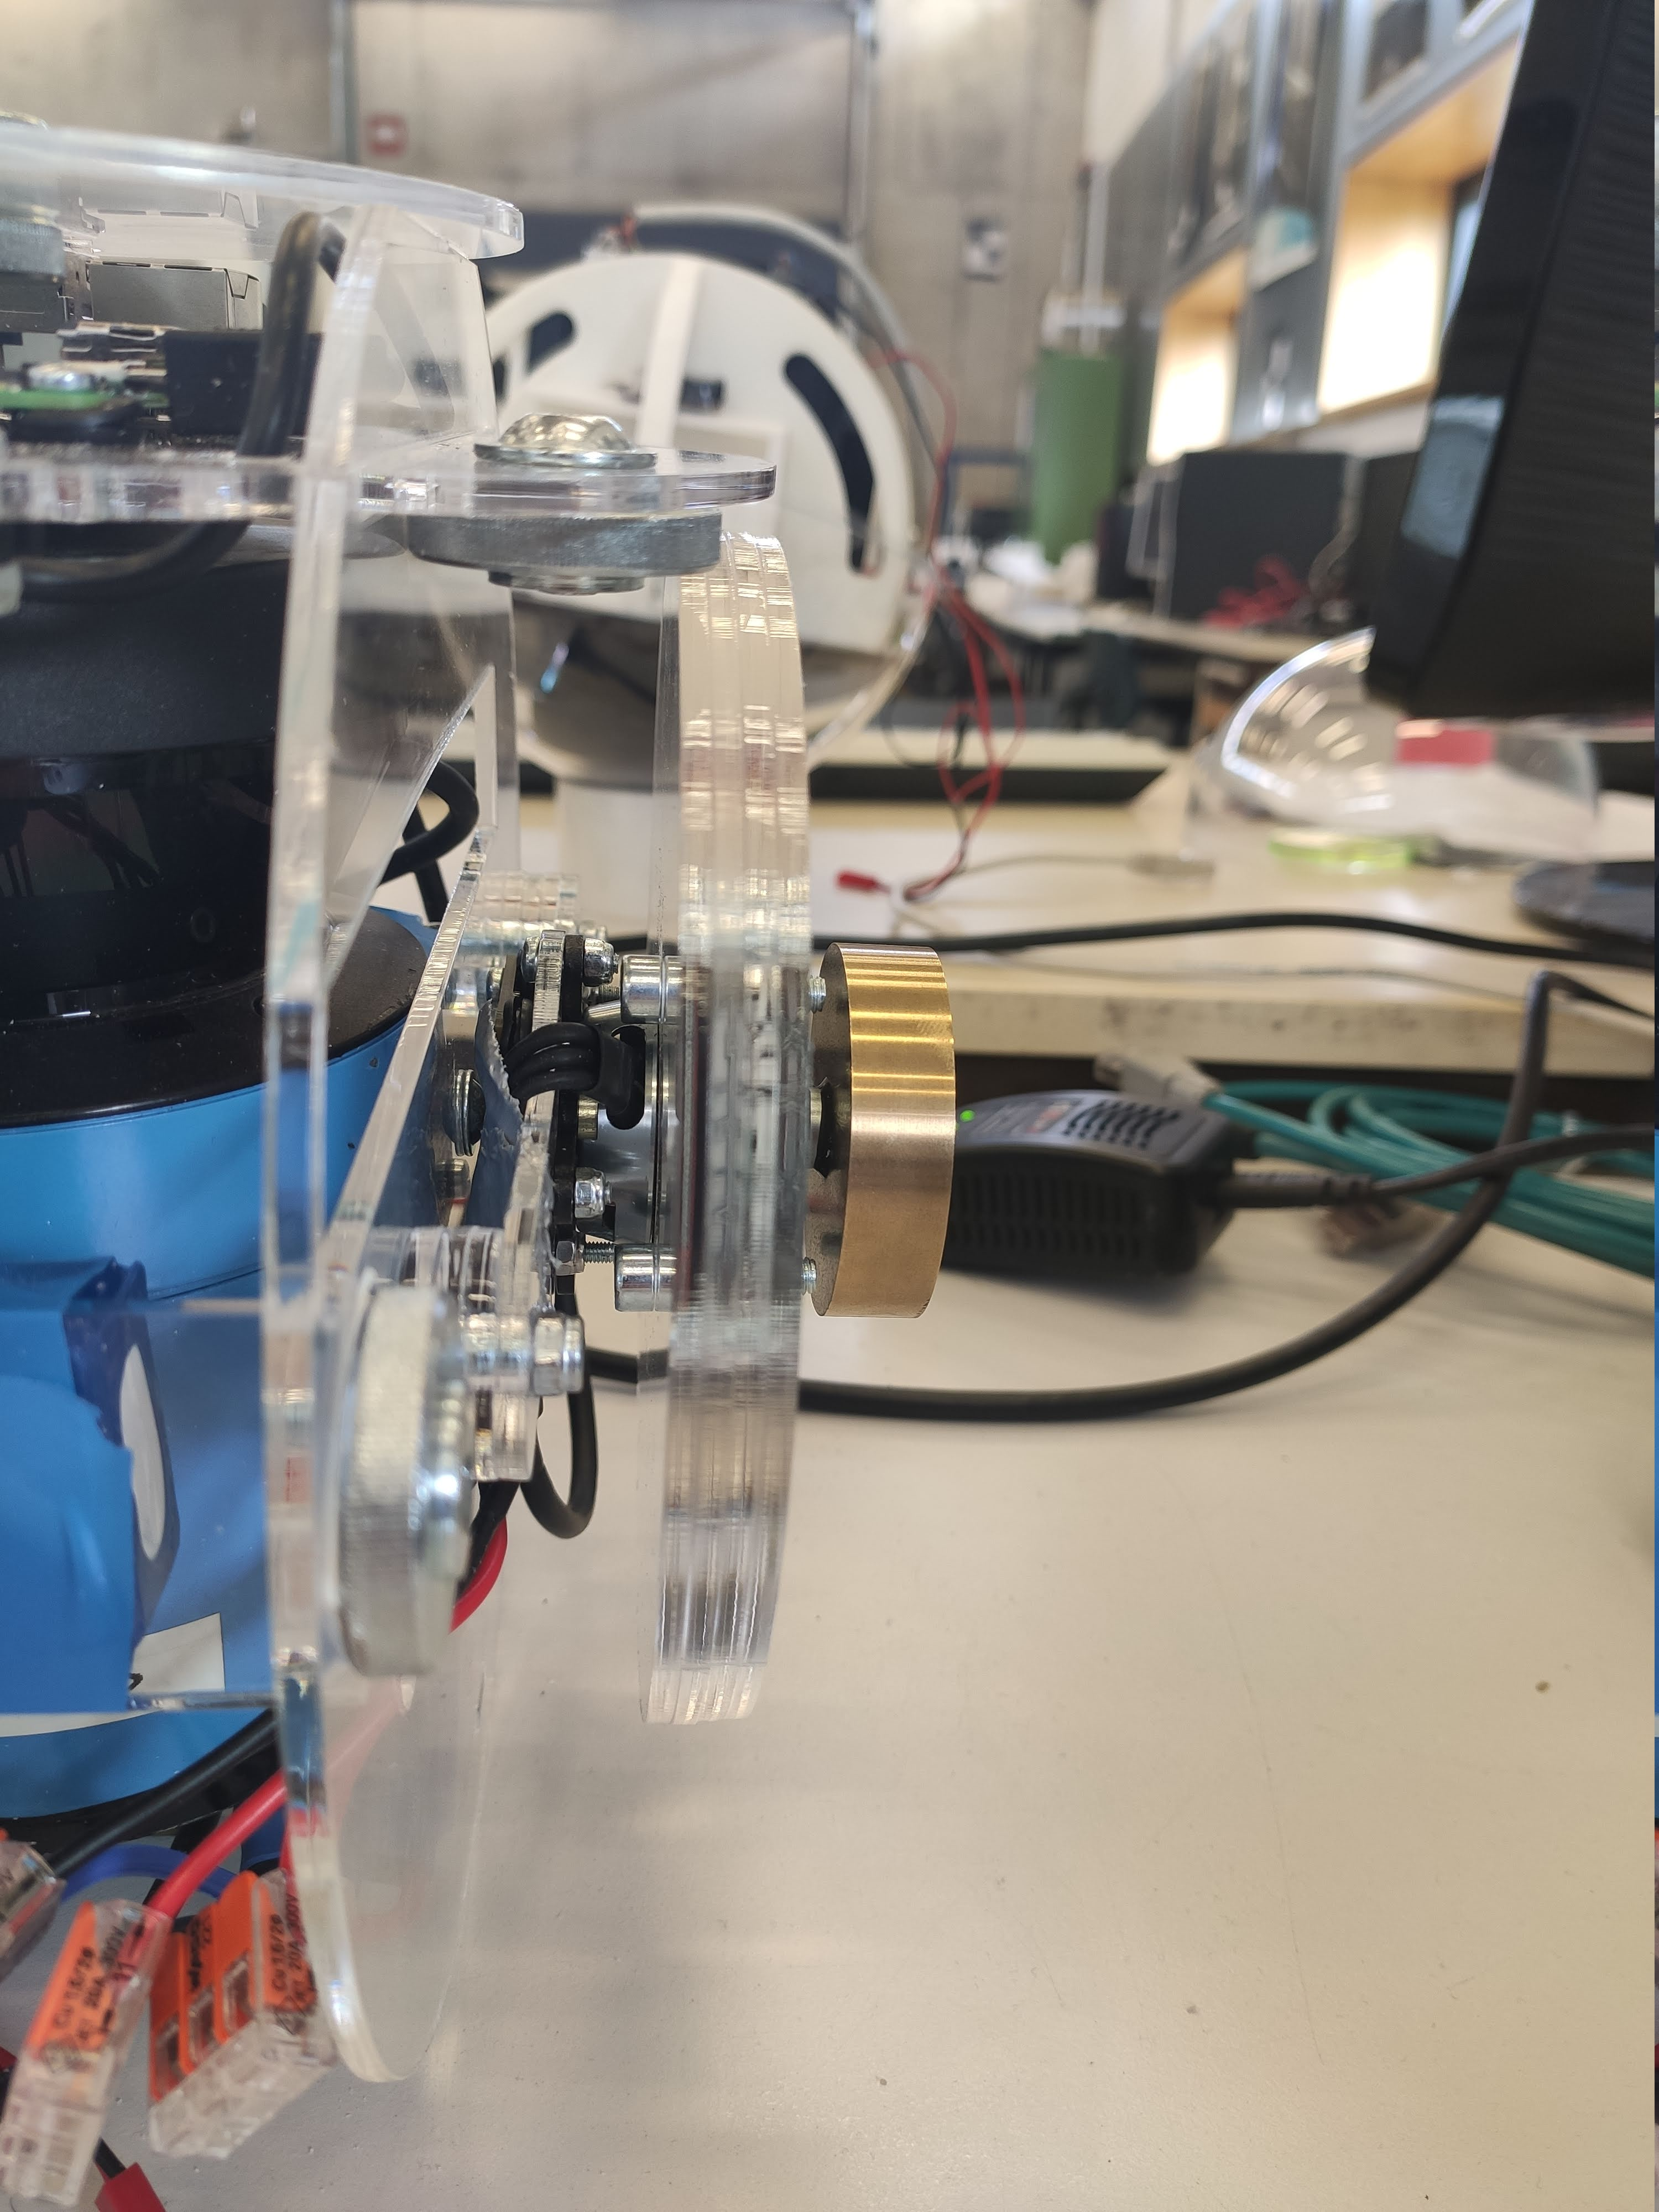
\includegraphics[height=50mm]{../Media/sphereRightMotor.jpg}   
\\\vspace{0.5cm}
\begin{subfigure}[b]{0.32\textwidth}
	\centering
	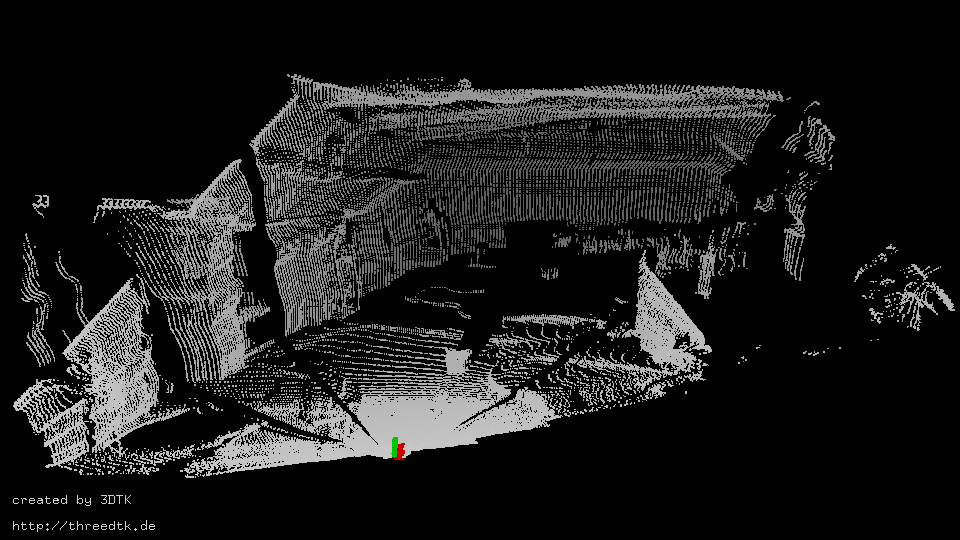
\includegraphics[width=\textwidth]{../Media/FirstDecentMap}
	\caption{Test with limited movement and no exterior shell.}
	\label{sec:experimentalResults:3DLaserScanning:fig:firstpointcloud}
\end{subfigure}
\begin{subfigure}[b]{0.32\textwidth}
	\centering
	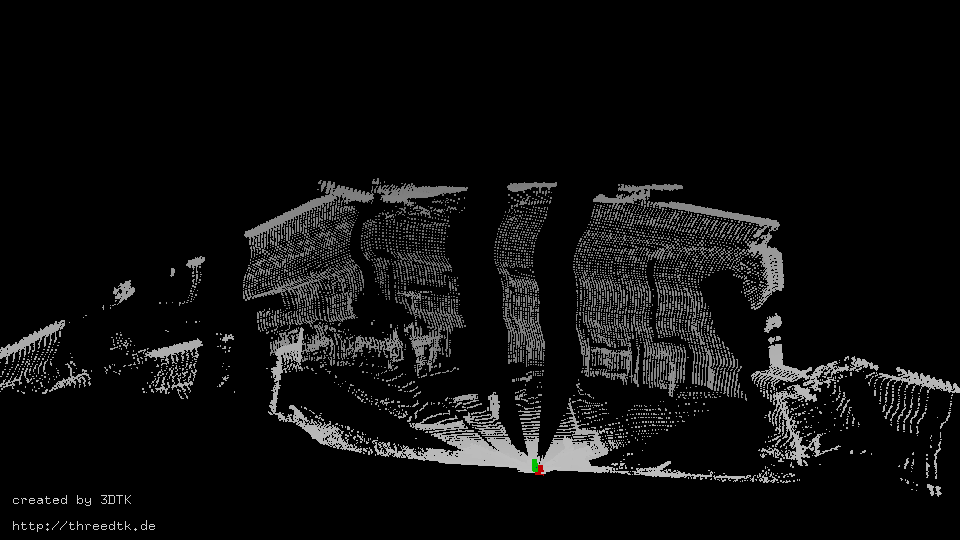
\includegraphics[width=\textwidth]{../Media/testScanWithTop}
	\caption{Test with limited movement and exterior shell.}
	\label{sec:experimentalResults:3DLaserScanning:fig:secondpointcloud}
\end{subfigure}
\begin{subfigure}[b]{0.32\textwidth}
	\centering
	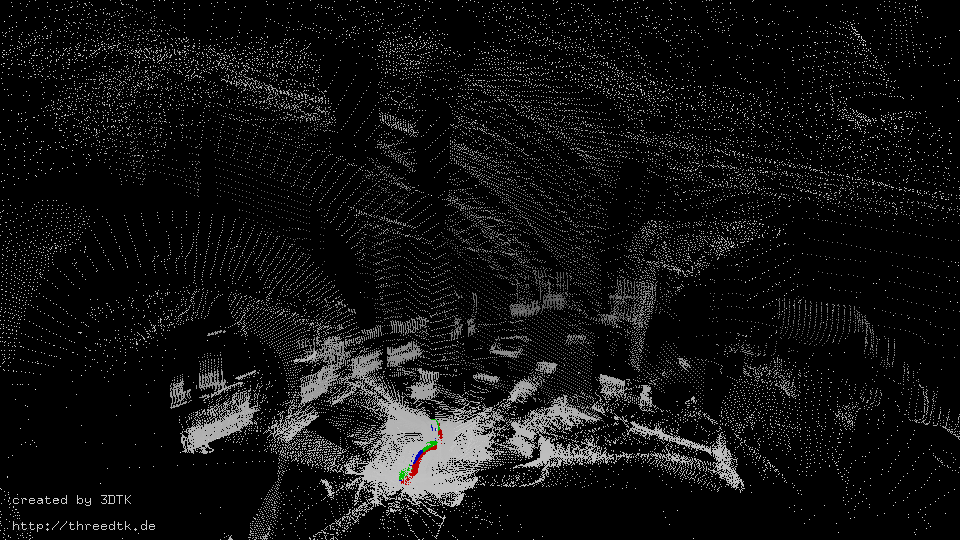
\includegraphics[width=\textwidth]{../Media/RollingTestMap}
	\caption{Test with exterior shell and full movement.}
	\label{sec:experimentalResults:3DLaserScanning:fig:thirdpointcloud}
\end{subfigure}
\caption{Hardware setup and laser-scanning Results of the L.U.N.A sphere prototype The Hardware including notches in the shell and friction granule (middle left). IMU (beneath supporting structure) and brushless motor  including flywheel mass (above supporting structure)(middle right).}
\label{sec:TechnicalApproach:fig:setup}

\end{figure}

\section{Experiments completed or scheduled}

All Experiments have been completed.\\

Multiple Basic-Roll-Tests: as the driving mechanism is not the common approach, where the rotation of a non-homogenus mass-distribution leads to the rotation, there where several basic tests for the driving mechanism conducted. \newline


Outdoor and indoor scanning-Tests: the environment-scanning was tested indoor and outdoor. 
\newline
Stress-Test for the micro-controller: evaluating the amount of required tasks capable by the micro-controller itself  and therefore scaling the need of an server-structure. \newline
Single-IMU vs Triple-IMU test: the difference between the use of a single IMU and the triple-IMU approach presented in 
\ref{sec:TechnicalApproach}  was tested.

\section{Main Experimental Insights}

The experiments lead to multiple hardware and software improvements
The impulse by conservation of angular momentum drive accelerates the L.U.N.A. sphere reliably.
Figure \ref{sec:technicalApproach:fig:angvel} shows the angular acceleration of the whole sphere measured by the IMU system in one test run. 
Furthermore, it shows that the acceleration along the rotational axis of the flywheels rises while the accelerations along the other axes remain lower, albeit are noisy. 
However, it also shows the decrease in noise due to the combination of the IMU measurements.
The vibrations and tilt of the robot contribute to the velocities along the other axes.
The vibrations are results of inexact drilling of the flywheels such that there is an unbalance.
At the main test site the ground is a hard, clean and low friction concrete floor.
In such a scenario the vibrations add up and lead to slippage.
However, a rubber surface (a running track) absorb the vibrations, such that the acceleration process happens reliably.\newline
Furthermore the tests regarding the laser-scanning showed the need of further improvement like re-positioning the laser-scanner and the need for cutting windows into the sphere.

\begin{figure}
\centering
\begin{subfigure}{0.45\textwidth}
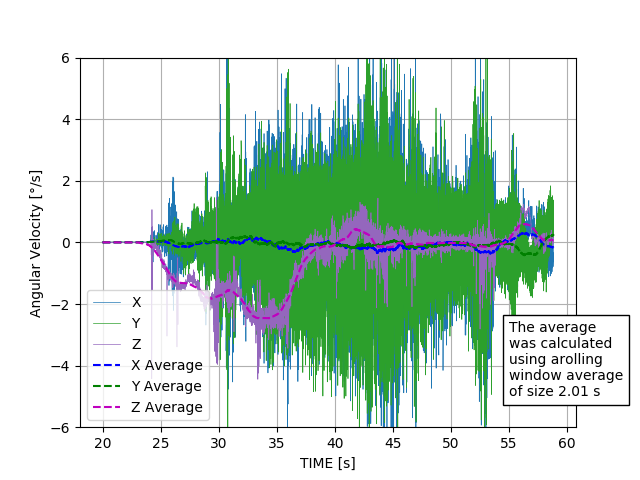
\includegraphics[width=\textwidth]{./plotsAndScripts/angVel-2020-01-29-16-14-54/imu1_ang_vel}
\caption{IMU 1: Z-Axis corresponds to Sphere X-Axis}
\label{sec:technicalApproach:fig:imu1_ang_vel}
\end{subfigure}\hfill
\begin{subfigure}{0.45\textwidth}
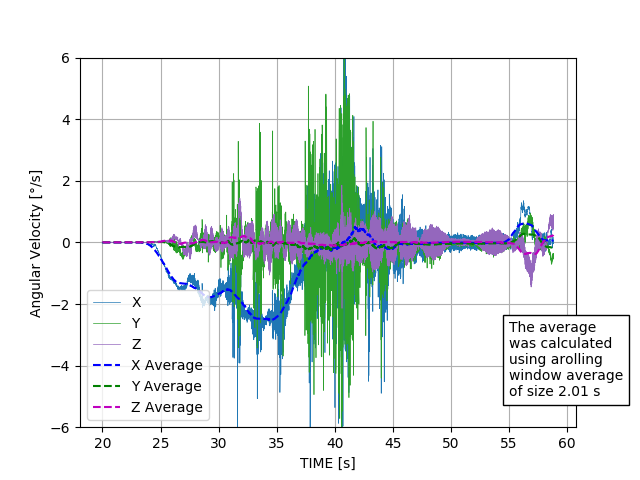
\includegraphics[width=\textwidth]{./plotsAndScripts/angVel-2020-01-29-16-14-54/imu2_ang_vel}
\caption{IMU 2: Z-Axis corresponds to Sphere Z-Axis}
\label{sec:technicalApproach:fig:imu2_ang_vel}
\end{subfigure}\hfill\\

\begin{subfigure}{0.45\textwidth}
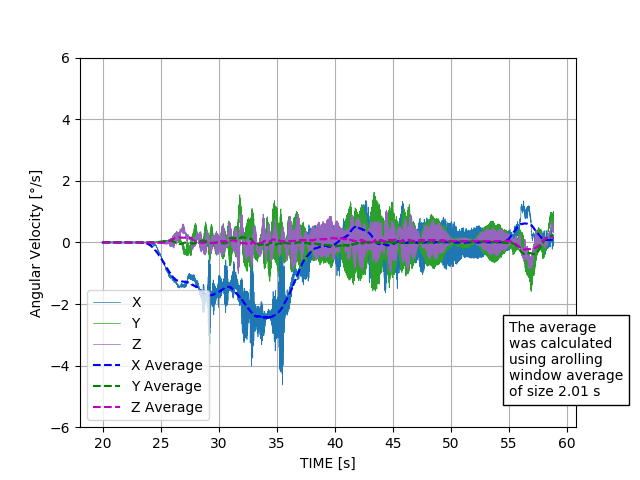
\includegraphics[width=\textwidth]{./plotsAndScripts/angVel-2020-01-29-16-14-54/imu3_ang_vel}
\caption{IMU 3: Z-Axis corresponds to Sphere Y-Axis}
\label{sec:technicalApproach:fig:imu3_ang_vel}
\end{subfigure}\hfill
\begin{subfigure}{0.45\textwidth}
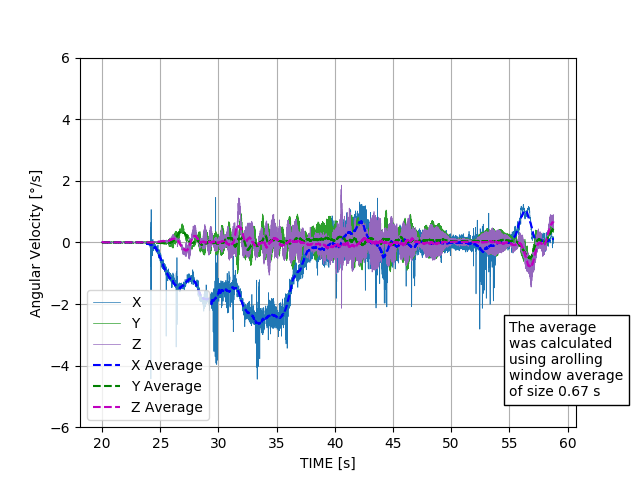
\includegraphics[width=\textwidth]{./plotsAndScripts/angVel-2020-01-29-16-14-54/merged_ang_vel}
\caption{Merged virtual IMU. Maps the Z-Axis of all other IMUs to the rotational axes.}
\label{sec:technicalApproach:fig:merged_ang_vel}
\end{subfigure}\hfill
\caption{Angular velocity measurements of singular IMUs and the combined IMU.}
\label{sec:technicalApproach:fig:angvel}
\end{figure}

\begin{acknowledgement}
The authors thank Dieter Ziegler and Sergio Montenegro for supporting our work and the Elite Network Bavaria for providing funding. 

\subsection*{Authors Note}
In an attempt to abide by the \href{https://www.go-fair.org/fair-principles}{Fair-Principles} of open science the authors provided all code developed and further information at their \href{https://github.com/fallow24/L.U.N.A}{GitHub} page.
\end{acknowledgement}

\bibliographystyle{plain}
\bibliography{andreas_publications}

\end{document}
